%%%%%%%%%%%%%%%%%%%%%%%%%%%%%%%%%%%%%%%%%
% Stylish Article
% LaTeX Template
% Version 2.1 (1/10/15)
%
% This template has been downloaded from:
% http://www.LaTeXTemplates.com
%
% Original author:
% Mathias Legrand (legrand.mathias@gmail.com) 
% With extensive modifications by:
% Vel (vel@latextemplates.com)
% Final ACS by:
% Juan Barbosa
% License:
% CC BY-NC-SA 3.0 (http://creativecommons.org/licenses/by-nc-sa/3.0/)
%
%%%%%%%%%%%%%%%%%%%%%%%%%%%%%%%%%%%%%%%%%
\documentclass[fleqn,10pt]{SelfArx}
%\usepackage[superscript]{cite}
\usepackage{wrapfig}
\usepackage{subcaption}
\usepackage[numbers, super]{natbib}
%----------------------------------------------------------------------------------------
%	ARTICLE INFORMATION
%----------------------------------------------------------------------------------------

\JournalInfo{Laboratorio Org\'anica 3, No. 3, 09/09/2017} % Journal information
\Archive{ }

\PaperTitle{Reacci\'on de Ozon\'olisis} %
%\Keywords{Keyword1 --- Keyword2 --- Keyword3} % Keywords - if you don't want any simply remove all the text between the curly brackets
%\newcommand{\keywordname}{Keywords} % Defines the keywords heading name

%----------------------------------------------------------------------------------------
%	ABSTRACT
%----------------------------------------------------------------------------------------

\Abstract{
\begin{wrapfigure}{r}{0.45\textwidth}
	\centering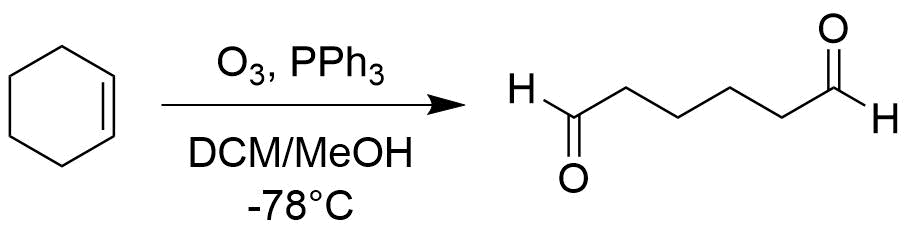
\includegraphics[width=0.9\linewidth]{structures/overall.png}
\end{wrapfigure}

La preparaci\'on de adipaldehído fue realizada a partir de ciclohexeno, en presencia de ozono y trifenilfosfina. El tiempo de reacci\'on fue inferior a los 10 minutos, el producto fue purificado en columna obteniendose un porcentaje de recuperaci\'on de \_\_\_ \% y un rendimiento de \_\_\_ \%. El producto fue caracterizado usando t\'ecnicas espectrosc\'opicas como $^1$HRMN y $^{13}$CRMN.
}

%----------------------------------------------------------------------------------------

\begin{document}

\flushbottom % Makes all text pages the same height

\maketitle % Print the title and abstract box

%\tableofcontents % Print the contents section

\thispagestyle{empty} % Removes page numbering from the first page



%----------------------------------------------------------------------------------------
%	ARTICLE CONTENTS
%----------------------------------------------------------------------------------------

\section*{Introducci\'on} % The \section*{} command stops section numbering
%------------------------------------------------
La ozon\'olisis represanta una importante reacci\'on oxidativa en la qu\'imica org\'anica. Como todas las reacciones de oxidaci\'on tienen una especial importancia en la qu\'imica, ya que permiten convertir grupos funcionales y preparar compuestos complejos a partir de reactivos simples. Si bien la definici\'on qu\'imica de oxidaci\'on involucra una transferencia de electrones en la cual la mol\'ecula o \'atomo oxidado pierde electrones, en la qu\'imica org\'anica la oxidaci\'on muchas veces implica el aumento de enlaces carbono-ox\'igeno en una mol\'ecula, aunque no es la \'unica forma de oxidaci\'on \cite{Gilbert2010}.

La mayor\'ia de las reacciones de los alquenos, transforman el enlace $\pi$ en un enlace $\sigma$ aprovechando la riqueza electr\'onica de los enlaces dobles. Los alquenos al igual que otros grupos funcionales presentan principalmente tres tipos de reacciones: adici\'on, eliminaci\'on y sustituci\'on, sin embargo tambi\'en existe la posibilidad de reacciones de ruptura: una reacci\'on donde el enlace $\pi$ se rompe y el alqueno se transforma en dos mol\'eulas m\'as peque\~nas. La reacci\'on de ozon\'olisis adem\'as de generar dos nuevos enlaces carbono-ox\'igeno, da lugar a la degradaci\'on de la mol\'ecula inicial, esto impl\'ica que se clasifica como una reacci\'on de oxidaci\'on y ruptura \cite{Wade2013}\cite{Morrison2002}.
\begin{scheme}[h]
	\centering
	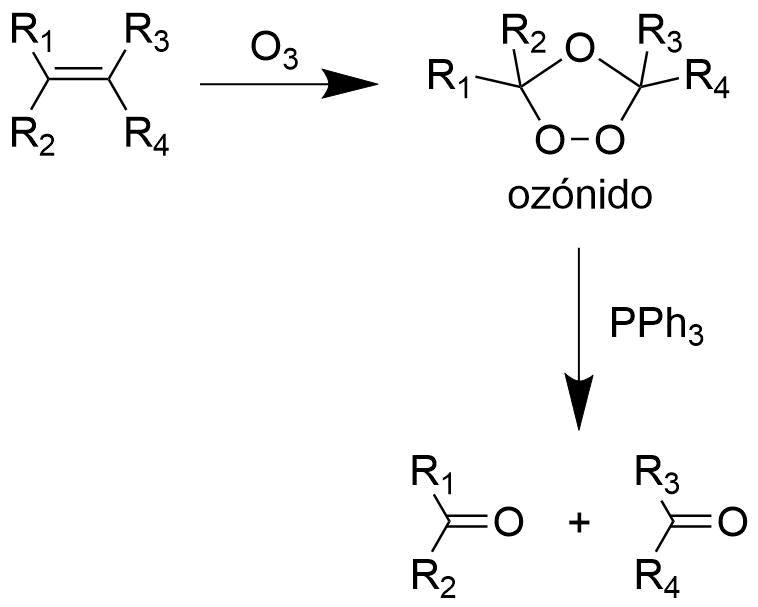
\includegraphics[width=0.7\linewidth]{structures/ozonolisis.png}
	\caption{Reacci\'on de ozonolisis \cite{Wade2013}.}
\end{scheme}

La reacci\'on de ozon\'olisis recibe su nombre debido a que la oxidaci\'on se lleva a cabo con ozono, el cual se adiciona sobre el doble enlace para formar un oz\'onido, seguido de la ruptura del alqueno \cite{Morrison2002}. El ozono es una mol\'ecula altamente reactiva, presenta 142 kJ/mol m\'as de energ\'ia comparada con el ox\'igeno molecular, parte de su reactividad obdece a la densidad de carga positiva sobre el ox\'igeno central \cite{Wade2013}.
\begin{figure}[h]
	\centering
	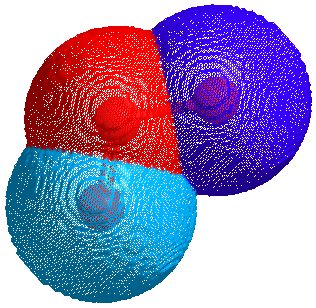
\includegraphics[width=0.5\linewidth]{structures/ozone.png}
	\caption{Densidades de carga en el ozono. De izquierda a derecha: -0.76$e$, 1.03$e$, -0.27$e$. Valores basados en el modelo de H\"uckel \cite{PerkinElmer}.}
\end{figure}
\section{Resultados y Discusi\'on}

\section{Conclusiones}
\section{Secci\'on experimental}

%----------------------------------------------------------------------------------------
%	REFERENCE LIST
%----------------------------------------------------------------------------------------
\phantomsection
\bibliography{informe}
\bibliographystyle{achemso}

%----------------------------------------------------------------------------------------
\newpage
\onecolumn
\section{Informaci\'on suplementaria}\label{sec: complementaria}
\begin{figure}[h]
	\centering
	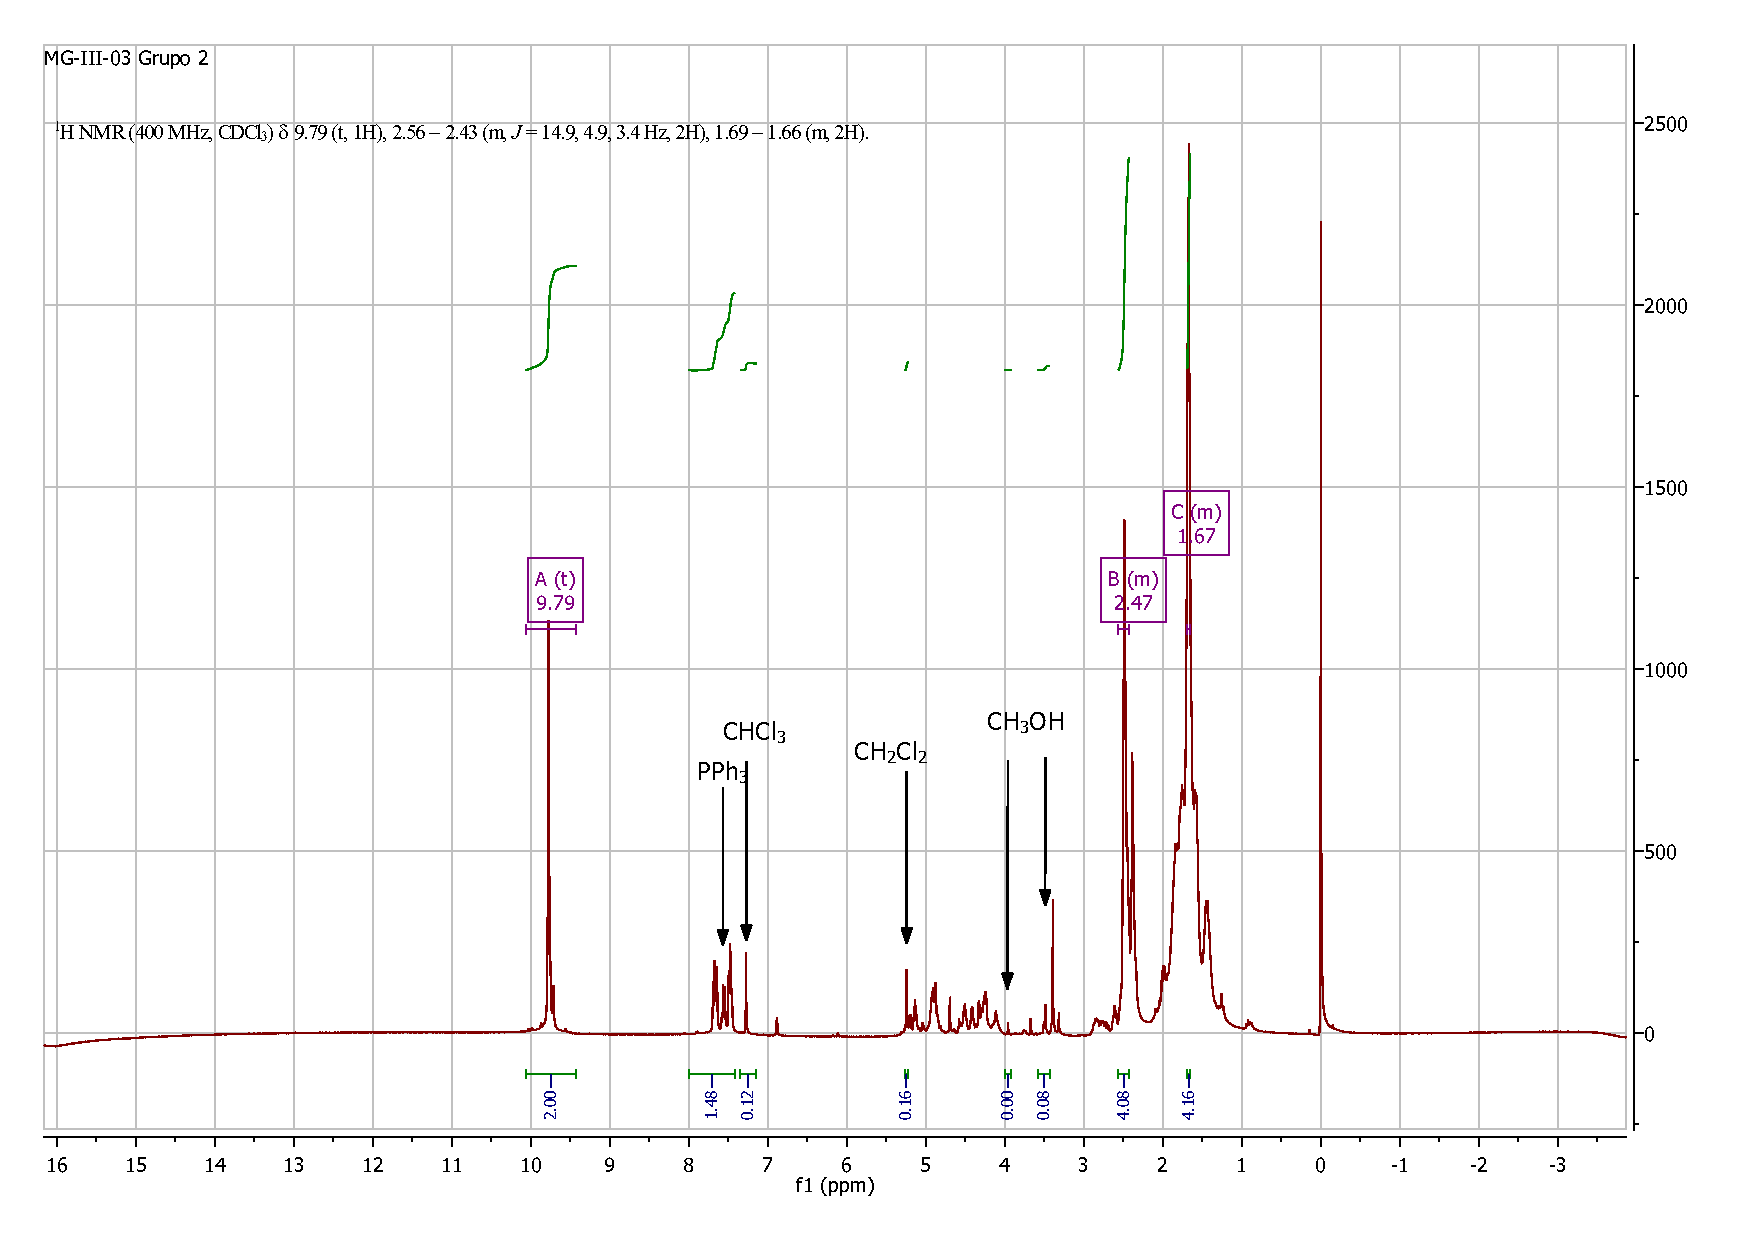
\includegraphics[width=0.5\textheight]{RMN/H.pdf}
	\caption{$^1$HRMN del producto purificado.}
\end{figure}
\begin{figure}[h]
	\centering
	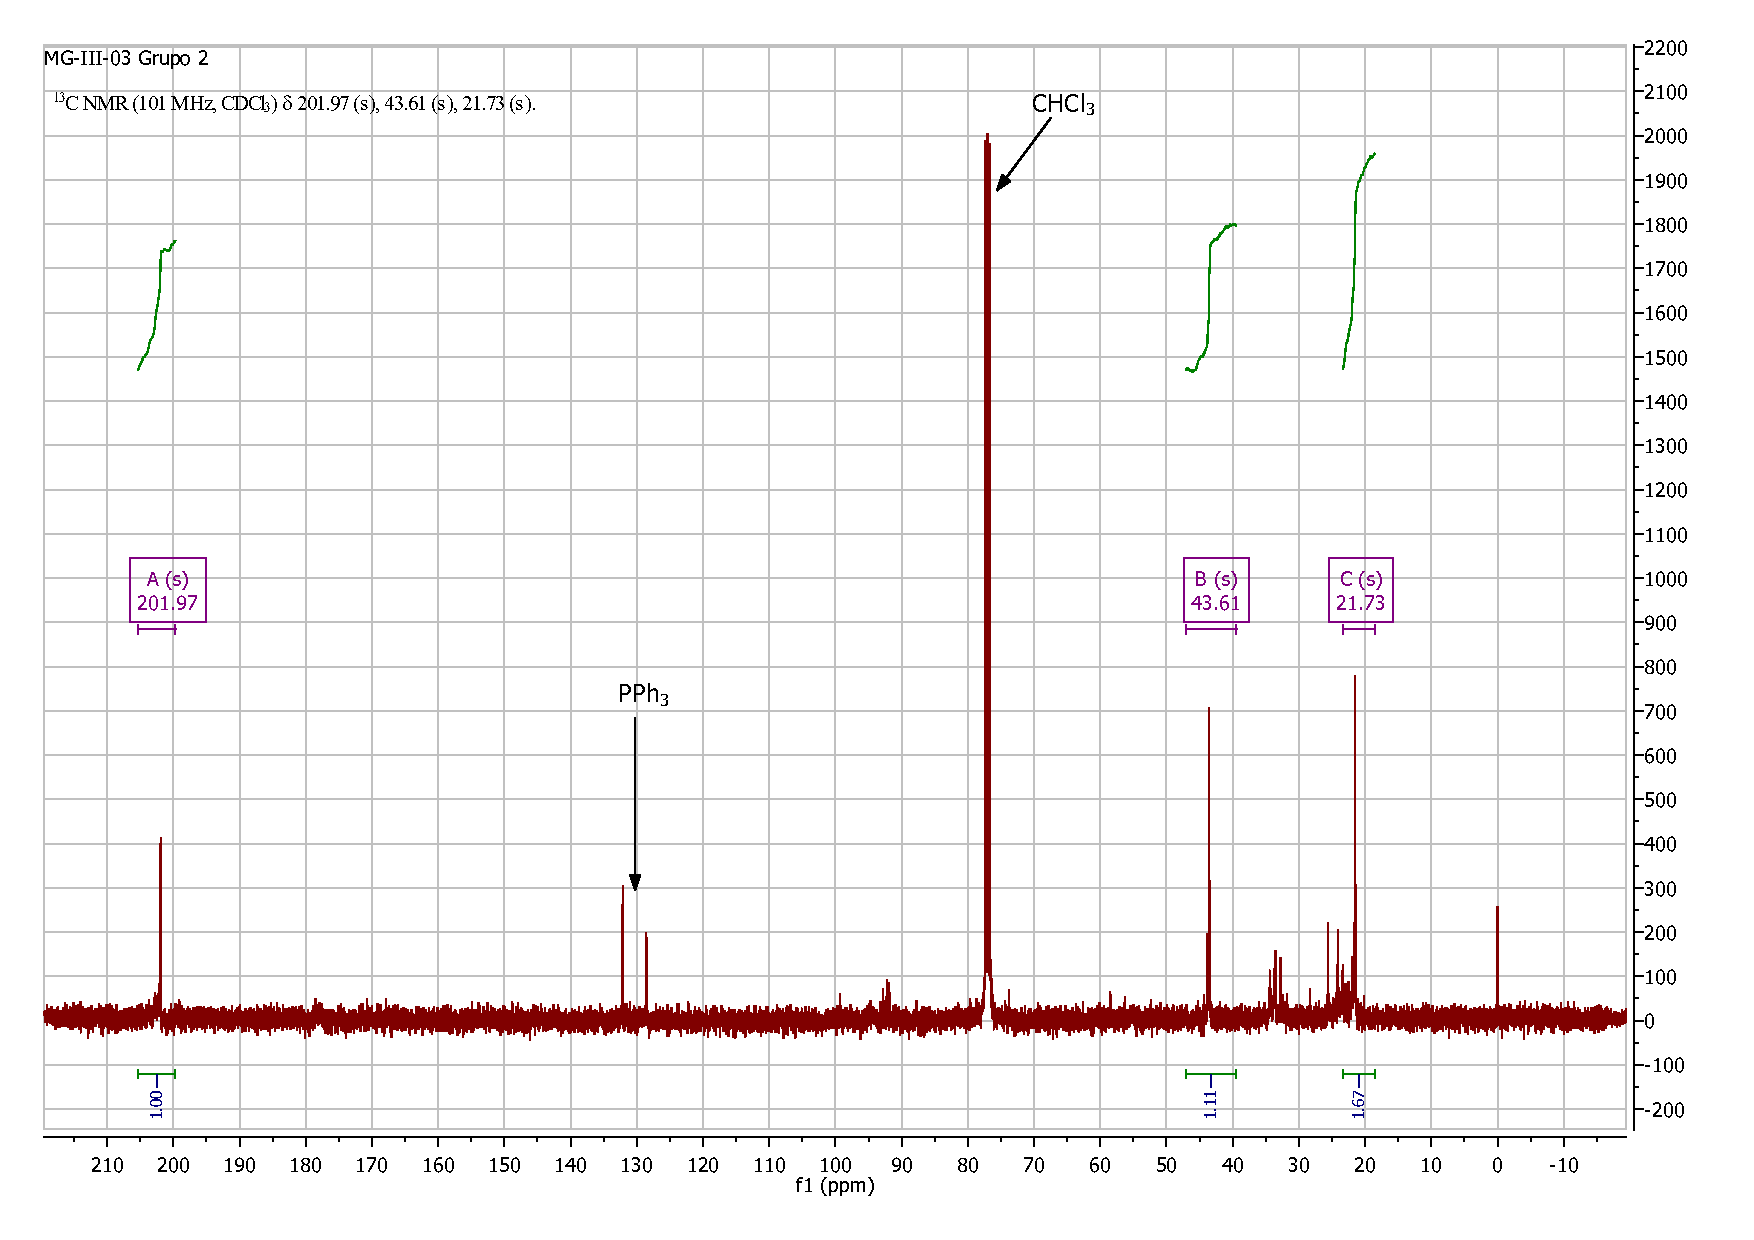
\includegraphics[width=0.5\textheight]{RMN/C.pdf}
	\caption{$^{13}$CRMN del producto purificado.}
\end{figure}
\end{document}